%%%%%%%%%%%%%%%%%%%%%%%%%%%%%%%%%%%%%%%%%
% Masters/Doctoral Thesis 
% LaTeX Template
% Version 2.5 (27/8/17)
%
% This template was downloaded from:
% http://www.LaTeXTemplates.com
%
% Version 2.x major modifications by:
% Vel (vel@latextemplates.com)
%
% This template is based on a template by:
% Steve Gunn (http://users.ecs.soton.ac.uk/srg/softwaretools/document/templates/)
% Sunil Patel (http://www.sunilpatel.co.uk/thesis-template/)
%
% Template license:
% CC BY-NC-SA 3.0 (http://creativecommons.org/licenses/by-nc-sa/3.0/)
%
%%%%%%%%%%%%%%%%%%%%%%%%%%%%%%%%%%%%%%%%%

%----------------------------------------------------------------------------------------
%	PACKAGES AND OTHER DOCUMENT CONFIGURATIONS
%----------------------------------------------------------------------------------------

\documentclass[
11pt, % The default document font size, options: 10pt, 11pt, 12pt
%oneside, % Two side (alternating margins) for binding by default, uncomment to switch to one side
english, % ngerman for German
singlespacing, % Single line spacing, alternatives: onehalfspacing or doublespacing
%draft, % Uncomment to enable draft mode (no pictures, no links, overfull hboxes indicated)
%nolistspacing, % If the document is onehalfspacing or doublespacing, uncomment this to set spacing in lists to single
%liststotoc, % Uncomment to add the list of figures/tables/etc to the table of contents
%toctotoc, % Uncomment to add the main table of contents to the table of contents
%parskip, % Uncomment to add space between paragraphs
%nohyperref, % Uncomment to not load the hyperref package
headsepline, % Uncomment to get a line under the header
%chapterinoneline, % Uncomment to place the chapter title next to the number on one line
%consistentlayout, % Uncomment to change the layout of the declaration, abstract and acknowledgements pages to match the default layout
]{MastersDoctoralThesis} % The class file specifying the document structure

\usepackage[utf8]{inputenc} % Required for inputting international characters
\usepackage[T1]{fontenc} % Output font encoding for international characters

\usepackage{mathpazo} % Use the Palatino font by default

\usepackage[backend=bibtex,style=authoryear,natbib=true]{biblatex} % Use the bibtex backend with the authoryear citation style (which resembles APA)

\addbibresource{example.bib} % The filename of the bibliography

\usepackage[autostyle=true]{csquotes} % Required to generate language-dependent quotes in the bibliography

%----------------------------------------------------------------------------------------
%	MARGIN SETTINGS
%----------------------------------------------------------------------------------------

\geometry{
	paper=a4paper, % Change to letterpaper for US letter
	inner=2.5cm, % Inner margin
	outer=3.8cm, % Outer margin
	bindingoffset=.5cm, % Binding offset
	top=1.5cm, % Top margin
	bottom=1.5cm, % Bottom margin
	%showframe, % Uncomment to show how the type block is set on the page
}

%----------------------------------------------------------------------------------------
%	THESIS INFORMATION
%----------------------------------------------------------------------------------------

\thesistitle{Proposals on Efficient Software Implementation of Pairing-Based Cryptographic Primitives} % Your thesis title, this is used in the title and abstract, print it elsewhere with \ttitle
\supervisor{Dr. Yasuyuki \textsc{Nogami}} % Your supervisor's name, this is used in the title page, print it elsewhere with \supname
\examiner{} % Your examiner's name, this is not currently used anywhere in the template, print it elsewhere with \examname
\degree{Doctor of Philosophy} % Your degree name, this is used in the title page and abstract, print it elsewhere with \degreename
\author{Md. Al-Amin \textsc{Khandaker}} % Your name, this is used in the title page and abstract, print it elsewhere with \authorname
\addresses{} % Your address, this is not currently used anywhere in the template, print it elsewhere with \addressname

\subject{Biological Sciences} % Your subject area, this is not currently used anywhere in the template, print it elsewhere with \subjectname
\keywords{} % Keywords for your thesis, this is not currently used anywhere in the template, print it elsewhere with \keywordnames
\university{\href{http://www.okayama-u.ac.jp}{Okayama University}} % Your university's name and URL, this is used in the title page and abstract, print it elsewhere with \univname
\department{\href{https://www.gnst.okayama-u.ac.jp}{Graduate School of Natural Science and Technology}} % Your department's name and URL, this is used in the title page and abstract, print it elsewhere with \deptname
\group{\href{http://isec.ec.okayama-u.ac.jp}{Information Security Lab.}} % Your research group's name and URL, this is used in the title page, print it elsewhere with \groupname
\faculty{\href{http://faculty.university.com}{Faculty of Engineering}} % Your faculty's name and URL, this is used in the title page and abstract, print it elsewhere with \facname

\AtBeginDocument{
\hypersetup{pdftitle=\ttitle} % Set the PDF's title to your title
\hypersetup{pdfauthor=\authorname} % Set the PDF's author to your name
\hypersetup{pdfkeywords=\keywordnames} % Set the PDF's keywords to your keywords
}

\begin{document}

\frontmatter % Use roman page numbering style (i, ii, iii, iv...) for the pre-content pages

\pagestyle{plain} % Default to the plain heading style until the thesis style is called for the body content

%----------------------------------------------------------------------------------------
%	TITLE PAGE
%----------------------------------------------------------------------------------------

\begin{titlepage}
\begin{center}

\vspace*{.06\textheight}
% {\scshape\LARGE \univname\par}\vspace{1.5cm} % University name
\textsc{\Large Doctoral Thesis}\\[0.5cm] % Thesis type

\HRule \\[0.4cm] % Horizontal line
{\huge \bfseries \ttitle\par}\vspace{0.4cm} % Thesis title
\HRule \\[1.5cm] % Horizontal line
 
\begin{minipage}[t]{0.4\textwidth}
\begin{flushleft} \large
\emph{Author:}\\
{\authorname} % Author name - remove the \href bracket to remove the link
\end{flushleft}
\end{minipage}
\begin{minipage}[t]{0.4\textwidth}
\begin{flushright} \large
\emph{Supervisor:} \\
\href{http://isec.ec.okayama-u.ac.jp/nogami}{\supname} % Supervisor name - remove the \href bracket to remove the link  
\end{flushright}
\end{minipage}\\[3cm]
 
\vfill

\large \textit{A thesis submitted in fulfillment of the requirements\\ for the degree of \degreename}\\[0.3cm] % University requirement text
\textit{in the}\\[0.4cm]
\groupname\\\deptname\\[2cm] % Research group name and department name
{\scshape\LARGE \univname\par}\vspace{1.5cm} % University name

\includegraphics[scale = 0.1]{okadailogo} \\ % \\ University/department logo - uncomment to place it
\vfill
{\large \today}\\[4cm] % Date
\vfill
\end{center}
\end{titlepage}

%----------------------------------------------------------------------------------------
%	DECLARATION PAGE
%----------------------------------------------------------------------------------------

\begin{declaration}
\addchaptertocentry{\authorshipname} % Add the declaration to the table of contents
\noindent I, \authorname, declare that this thesis titled, \enquote{\ttitle} and the work presented in it are my own. I confirm that:

\begin{itemize} 
\item This work was done wholly or mainly while in candidature for a research degree at this University.
\item Where any part of this thesis has previously been submitted for a degree or any other qualification at this University or any other institution, this has been clearly stated.
\item Where I have consulted the published work of others, this is always clearly attributed.
\item Where I have quoted from the work of others, the source is always given. With the exception of such quotations, this thesis is entirely my own work.
\item I have acknowledged all main sources of help.
\item Where the thesis is based on work done by myself jointly with others, I have made clear exactly what was done by others and what I have contributed myself.\\
\end{itemize}
 
\noindent Signed:\\
\rule[0.5em]{25em}{0.5pt} % This prints a line for the signature
 
\noindent Date:\\
\rule[0.5em]{25em}{0.5pt} % This prints a line to write the date
\end{declaration}

\cleardoublepage

%----------------------------------------------------------------------------------------
%	QUOTATION PAGE
%----------------------------------------------------------------------------------------

\vspace*{0.2\textheight}

\noindent\enquote{\itshape Thanks to my solid academic training, today I can write hundreds of words on virtually any topic without possessing a shred of information, which is how I got a good job in journalism.}\bigbreak

\hfill Dave Barry

%----------------------------------------------------------------------------------------
%	ABSTRACT PAGE
%----------------------------------------------------------------------------------------

\begin{abstract}
\addchaptertocentry{\abstractname} % Add the abstract to the table of contents
The Thesis Abstract is written here (and usually kept to just this page). The page is kept centered vertically so can expand into the blank space above the title too\ldots
\end{abstract}

%----------------------------------------------------------------------------------------
%	ACKNOWLEDGEMENTS
%----------------------------------------------------------------------------------------

\begin{acknowledgements}
\addchaptertocentry{\acknowledgementname} % Add the acknowledgements to the table of contents
The acknowledgments and the people to thank go here, don't forget to include your project advisor\ldots
\end{acknowledgements}

%----------------------------------------------------------------------------------------
%	LIST OF CONTENTS/FIGURES/TABLES PAGES
%----------------------------------------------------------------------------------------

\tableofcontents % Prints the main table of contents

\listoffigures % Prints the list of figures

\listoftables % Prints the list of tables

%----------------------------------------------------------------------------------------
%	ABBREVIATIONS
%----------------------------------------------------------------------------------------

\begin{abbreviations}{ll} % Include a list of abbreviations (a table of two columns)

\textbf{LAH} & \textbf{L}ist \textbf{A}bbreviations \textbf{H}ere\\
\textbf{WSF} & \textbf{W}hat (it) \textbf{S}tands \textbf{F}or\\

\end{abbreviations}

%----------------------------------------------------------------------------------------
%	PHYSICAL CONSTANTS/OTHER DEFINITIONS
%----------------------------------------------------------------------------------------

\begin{constants}{lr@{${}={}$}l} % The list of physical constants is a three column table

% The \SI{}{} command is provided by the siunitx package, see its documentation for instructions on how to use it

Speed of Light & $c_{0}$ & \SI{2.99792458e8}{\meter\per\second} (exact)\\
%Constant Name & $Symbol$ & $Constant Value$ with units\\

\end{constants}

%----------------------------------------------------------------------------------------
%	SYMBOLS
%----------------------------------------------------------------------------------------

\begin{symbols}{lll} % Include a list of Symbols (a three column table)

$a$ & distance & \si{\meter} \\
$P$ & power & \si{\watt} (\si{\joule\per\second}) \\
%Symbol & Name & Unit \\

\addlinespace % Gap to separate the Roman symbols from the Greek

$\omega$ & angular frequency & \si{\radian} \\

\end{symbols}

%----------------------------------------------------------------------------------------
%	DEDICATION
%----------------------------------------------------------------------------------------

\dedicatory{For/Dedicated to/To my\ldots} 

%----------------------------------------------------------------------------------------
%	THESIS CONTENT - CHAPTERS
%----------------------------------------------------------------------------------------

\mainmatter % Begin numeric (1,2,3...) page numbering

\pagestyle{thesis} % Return the page headers back to the "thesis" style

% Include the chapters of the thesis as separate files from the Chapters folder
% Uncomment the lines as you write the chapters

\chapter{Introduction}
\label{chap:Introduction}
This chapter introduces the related literature review, motivation, and goals of the undertaken research.
The chapter begins with a brief preface of cryptology and its importance in the era Internet of Things (IoT) and Big Data.
In \secref{ch1_subsec_pkc} we present how Public-Key Cryptography (PKC) is shaping the security of our everyday life.
We introduce the importance of Pairing-Based Cryptography (PBC) in \secref{ch1_subsec_pbc} for the next generation of security protocols. 
\secref{ch1_sec_motivation} presents the motivation behind the works undertaken to assemble of this thesis.
\secref{ch1_sec_outline} outlines the overall organization of this thesis.

\section{Cryptology}
\label{chap:sec:crypto}
Cryptography is the science of communicating with the authentic receiver through an insecure channel in secret. 
Cryptanalysis is the techniques of breaking the secret communications.
Cryptology is the combination of these two domains.

The history of cryptography dates back to the time of the Greek and Roman empire.
Julius Caesar used a simple shift and substitute system.
Up until the early '70s of the last century, cryptology was evolved mostly for military purposes. 
The cryptography got its first democratic form in 1975 when Diffie and Hellman invented the concept of public-key cryptography \cite{diffie1976new}. 
The concept was first realized by as practical cryptosystem by the works of Rivest, Shamir and Adleman (RSA) in 1977 \cite{rivest1978method}.
At the same time in 1977, National Bureau of Standards published a cryptosystem intended for the governmental agencies or banks with the named Data Encryption Standard (DES).
From then a new era of cryptography known as \textit{Modern cryptography} was initiated.
The well-organized procedures called \textit{protocols} is the basis of Modern cryptography.
One of the most elegant features of modern crypto-protocols is their inner algorithms are not secret yet withstand cryptanalysis from experts/attackers.
More importantly, these protocols are easy to use for people with no understanding of the underlying principles.
For example, paying by credit cards or withdrawing money using debit cards with a personal identification number (PIN) is doable without concerning what’s going on under the hood. 

The little basic functionality of modern cryptosystem is to enable a sender (Alice \footnote{Alice and Bob are fictional characters first used by Rivest, Shamir and Adleman in \cite{rivest1978method} as placeholder name in cryptology.}) to convert a message (plaintext) into a cipher (ciphertext) before sending to a legitimate receiver (Bob) over the public communication media. 
The receiver can convert the cipher back into the original message using secret information named as a key.
An adversary (Eve) eavesdrops in the middle of the conversation to retrieve information from the cipher.
The cipher is safe from to the adversary until the key is not compromised. 

The security of modern cryptosystems depends not on the secrecy of the encryption algorithms but the difficulty of one-way problems. 
Such problems are easy to calculate in one direction but practically impossible to calculate in reverse direction in a reasonable amount of time using reasonable resources.
For example, let us consider a ciphertext $\cal{C}$ and a plaintext $\cal{P}$ and a 128-bit key $\cal{K}$. 
The encryption scheme $\cal{E}$ takes input $\cal{P}$ and $\cal{K}$ and output $\cal{C}=E( \cal{P}, K)$. 
To obtain the  key $\cal{K}$ from the $(\cal{P,C})$ pair, we need to try $2^{128} = 340,282,366,920,938,463,463,374,607,431,768,211,456 \approx 3.4 \times 10^{38}$ (39 decimal digits) combination of $128$-bit keys.
The most potent supercomputer till this date can compute 122.3 PETA ($10^{15}$) floating-point operations per second (PFLOPS).
Let us consider an optimistic assumption that 1000 (FLOPS) is required to check one key combination.
Under this assumption, the supercomputer can compute $122.3. \times 10^{15} / 1000 = 122.3 \times 10^{12}$ key combinations per second.
Then it will take about $3.4 \times 10^{38}/((122.3 \times 10^{12})(365 \times 24 \times 60 \times 60)) \approx  8.8 \times 10^{16}$ earth years.
According to the standard model of physical cosmology \cite{Ade:2015xua} the age of our universe is $13.8 \time 10^9$ or 13.8 billion years. 
It means finding a key using brute force search will require $6.3$ million years more than the age of the universe.
We can imagine how big the number $2^{128}$ is from this comparison.

Cryptography became more important as individuals and business increasingly depend on the Internet as a channel for communication. Therefore, the following four properties are the basis of a cryptosystem.


\begin{itemize}
\item Data confidentiality:
This property ensures that confidential information such as bank transactions or medical data etc. are secret from unauthorized entities. 

\item Data integrity:
When data is stored, this property ensures that it not only kept secret (Data confidentiality) but also not rigged.
Confidentiality and integrity is enforced by encryption.

\item Authentication:
In connection-oriented communication, authentication proves both parties identity before communication begins.
The digital signature is used for this purpose to sign a message electronically.
It shields the legitimate party against masquerader from impersonating as a trusted party.
This property gives the receiver a confidence to believe that the actual signee indeed sends the message sent over the insecure channel.

\item Non repudiation:
Non-repudiation (with proof of origin and with proof of receipt) ensures that the sender and receiver can not deny having taken part in communication.
Non-repudiation is essential for many cases especially e-commerce while communicating over the Internet.
\end{itemize}

The modern crypto-protocols fall into the following two major categories. 

\subsection{Symmetric/Private-Key Cryptography}
Private-Key Cryptography, also known Symmetric Cryptography is the technique where both the sender and the receiver use the same \textit{key} or easily derivable from one another to encrypt and decrypt a message.
This type of cryptography has an ancient history. 

Modern cryptosystems offer efficient symmetric cryptography algorithms, e.g Advanced Encryption Standard (AES) \cite{AES_DaemenR02}.
Such cryptography has two main obstacles i.e. \textit{Key management} and \textit{key establishment}.
Since the keys are same, they need to keep private (\textit{Key management})  in both ends and should be shared securely beforehand (\textit{Key establishment}) without physically meeting.

The Public-key Cryptography offers the solution for \textit{Key establishment} applying Diffie-Hellman key exchange.
This work primarily focuses on a specific type of Public-key Cryptography. 
The subsequent chapters will describe in details.

\subsection{Public-key Cryptography}
\label{ch1_subsec_pkc}
The inception of public-key cryptography solved the problem of key distribution of Symmetric-key cryptography.
It is also known as Asymmetric Cryptography.
The basic idea of public-key cryptography is to use two different keys for each communicating party.
One key is public-key which can be used by anyone to encrypt the message. 
The receiver needs the correlated private key to decrypt the message.
From a given public key and ciphertext it is asymptotically difficult to obtain the private key.

As aforementioned, In 1976, Whitfield Diffie and Martin Hellman published their monumental work as a key exchange  protocol\cite{diffie1976new}.  
\fgref{fig_DHKE} shows the simple overview of the Diffie-Hellman Key Exchange (DHKE).
The problems of key distribution and storage associated with symmetric cryptography were the motivation behind the concept of Asymmetric Cryptography, also referred to as Public- Key Cryptography. 

In brief, the protocol has two public parameters, the prime number $p$ and a generator $g$ known to all the parties involved in the communication.
The main idea is of this protocol is based on the difficulty to solve the one-way function, i.e., discrete logarithm.
Let's say, it is easy to calculate Alice public key $k_A$ using Alice private key $k_{Ad}$ as $k_A = g^{k_{Ad}} (\bmod ~p).$ 
However, it will be difficult to obtain $k_{Ad}$ from $k_A, g$ and $p$.
In other words, it is easy to calculate the public key from the private key, but the reverse process is practically impossible.
Using this key-exchange, we change to establish a shared secret which we can for further encrypted communication.

  \begin{figure}
	\centering
	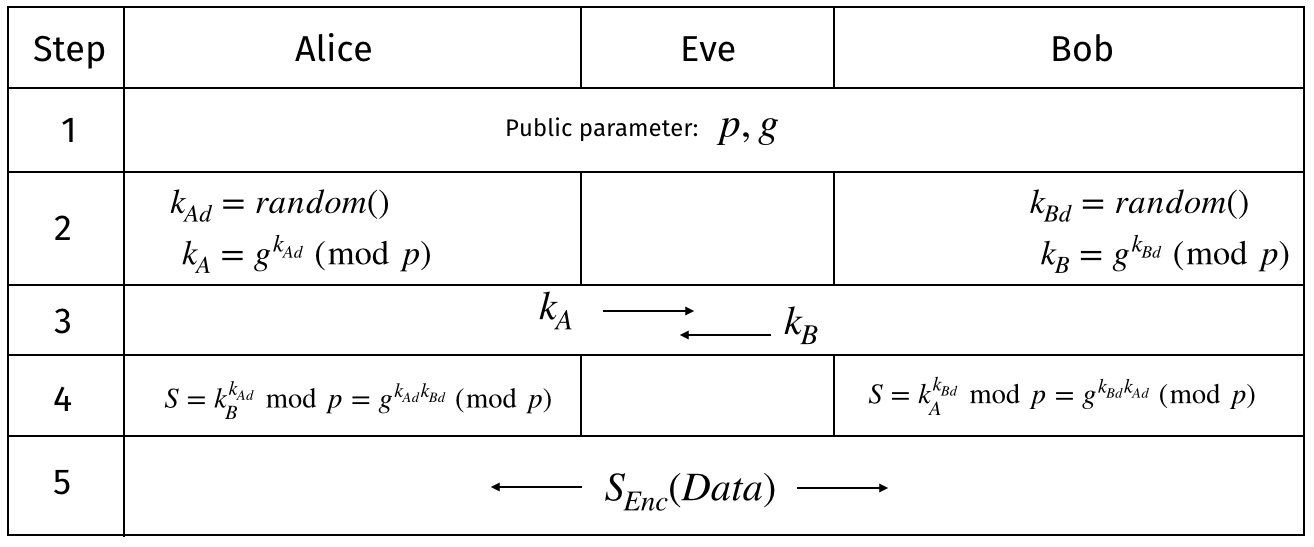
\includegraphics[width=.9\linewidth, height=.67\textheight, keepaspectratio]{Figures/DHKE}
	\caption{Exchanging shared secret key using DH-key exchange.}
	\label{fig_DHKE}
\end{figure}

Rivest, Shamir, and Adleman (RSA) realized this protocol in 1977 and published their magnum opus which is widely known as RSA cryptosystem \cite{rivest1978method}. 
The security of the RSA depends on the difficulty of factorization of a larger integer into its two prime factors and the trapdoor permutation for encryption.
Let us denote two large primes $p$ and $q$ (in practice about 1000-bit).
It is easy to calculate their product to get $n = pq$.
The reverse process that is for a given integer $n$ it will be arduous to retain $p$ and $q$.
Using the state-of-the-art integer factoring algorithm \textit{general number field sieve }(GNFS), it will take approximately $2^{90}$ basic operation to factor a 2048-bit integer.
After more than 40 years of the RSA breakthrough, it is still standing as an epitome of public key cryptography.
Besides encryption, RSA also enables \textit{digital signature }where the sender uses his private key to sign a message, and the receiver verifies the signature by the senders public key. 
Verification of a digitally signed message gives the receiver the confidence that a senders private key is tied to his public key.
It is done to prevent forgery and holds \textit{Non-repudiation} property.

In the mid 80's the independent work of Miller \cite{C:Miller85} and Koblitz \cite{koblitz1987elliptic} began the journey of elliptic curve cryptosystems (ECC). 
The security of elliptic curve cryptography protocols depends on the difficulty to solve elliptic curve discrete logarithm problem.
The mathematical details of this problem appear in Chapter 2. %TODO
ECC provides a shorter key length for the same level of security than RSA which makes ECC  popular among the researchers. 
Compared to RSA, ECC has other advantages. 
While RSA provides encryption and digital signature; ECC has a family of algorithms for encryption, signature, key agreement and some advanced high-level cryptographic protocols such as ID-based encryption \cite{AC:BonLynSha01}, where user's unique ID, e.g. email address, can be used as a public key. 
The high-level cryptographic functionalities are provided by paring over elliptic curves \cite{book_GPCMrabet2016} which brings a new paradigm in cryptography called pairing-based cryptography.

\subsection{Pairing-Based Cryptography}
\label{ch1_subsec_pbc}
Since the inception by Sakai et al. \cite{sakai2000cryptosystems}, pairing-based cryptography has gained much attention to cryptographic researchers as well as  to mathematicians. It gives flexibility to protocol researcher to innovate applications with provable security and at the same time to mathematicians and cryptography engineers to find efficient algorithms to make pairing implementation more efficient and practical.

Generally, a pairing is a bilinear map $e$ typically defined as  $\g1 \times \g2 \to \g3$, where $\g1$ and $\g2$ are additive cyclic sub-groups of  order $r$  on a certain elliptic curve $E$ over a finite extension field $\FPK$ and $\g3$ is a multiplicative cyclic group of order $r$ in $\mF{p}{k}$.
Let $E(\Fp)$ be the set of rational points over the prime field $\Fp$ which forms an additive Abelian group together with the point at infinity $\cal{O}$. The total number of rational points is denoted as $\#E(\Fp)$. Here, the order $r$ is a large prime number such that $r | \#E(\Fp)$ and gcd$(r,p)=1$. The embedding degree $k$ is the smallest positive integer such that $r | (p^k -1)$.
Two fundamental properties of pairing are
\begin{itemize}
	\item bilinearity is such that $\forall P_i \in \g1$ and $\forall Q_i \in \g2$, where $i= 1, 2$, then $e(Q_1+Q_2,P_1) = e(Q_1,P_1). e(Q_2,P_1)$ and $e(Q_1,P_1+P_2) = e(Q_1,P_1). e(Q_1,P_2)$,
	\item and $e$ is non-degenerate means $\forall P \in \g1$ there is a $Q \in \g2$ such that  $e(Q,P) \neq 1$ and $\forall Q \in \g2$ there is a $P \in \g1$ such that $e(P,Q) \neq 1$.
\end{itemize}
Such properties allows researchers to come up with various cryptographic applications including ID-based encryption \cite{C:BonFra01}, group signature authentication \cite{C:BonBoySha04}, and functional encryption \cite{C:OkaTak10}.  However, the security of pairing-based cryptosystems depends  on 
\begin{itemize}
	\item  the difficulty of solving elliptic curve discrete logarithm problem (ECDLP) in the groups of order $r$ over $\Fp$,
	\item  the infeasibility of solving the discrete logarithm problem (DLP) in the multiplicative group $\g3 \in \mF{p}{k}$,
	\item and the difficulty of pairing inversion.
\end{itemize}
To maintain the same security level in both groups, the size of the order $r$ and extension field $p^k$ is chosen accordingly. If the desired security level is $\delta$ then $\log_2 r  \geq 2\delta$ is desirable due to Pollard's rho algorithm \cite{1978-pollard-kangaroo}.  For efficient pairing, the ratio $\rho = \log_2 p^k/ \log_2 r \approx 1$,   is expected (usually  $1\leq  \rho  \leq 2$). In practice, elliptic curves with small embedding degrees $k$ and large $r$ are selected and commonly are knows as ``pairing-friendly" elliptic curves.

Galbraith et al. \cite{galbraith2008pairings} have classified pairings as three major categories based on the underlying group's structure as 
\begin{itemize}
	\item Type 1, where $\g1 = \g2$, also known as symmetric pairing. 
	\item Type 2, where $\g1 \neq \g2$, known as asymmetric pairing. There exists an efficiently computable isomorphism $\psi : \g2 \to \g1$ but none in reverse direction.
	\item Type 3, which is also asymmetric pairing, i.e., $\g1 \neq \g2$. But no efficiently computable isomorphism is known in either direction  between $\g1$ and $\g2$.
\end{itemize}


%This thesis chooses one of the Type 3 variants of pairing named as Optimal-Ate \cite{DBLP:journals/tit/Vercauteren10} with Kachisa-Schaefer-Scott (KSS) \cite{EPRINT:KacSchSco07} pairing-friendly curve of embedding degree $k=16$. 
%Few previous works have been done on this  curve. 
%Zhang et al. \cite{INDOCRYPT:ZhaLin12} have shown the computational estimation of the Miller's loop and proposed efficient final exponentiation for 192-bit security level in the context of Optimal-Ate pairing over KSS-16 curve. 
%A few years later Ghammam et al. \cite{EPRINT:GhaFou16b} have shown that KSS-16 is the best suited for multi-pairing (i.e., the product and/or the quotient) when the number of pairing is more than two. 
%Ghammam et al. \cite{EPRINT:GhaFou16b} also corrected the flaws of proposed final exponentiation algorithm by Zhang et al. \cite{INDOCRYPT:ZhaLin12} and proposed a new one and showed the vulnerability of Zhang's parameter settings against small subgroup attack. 
%The recent development of NFS by Kim and Barbulescu \cite{C:KimBar16} requires updating the parameter selection for all the existing pairings over the well known pairing-friendly curve families such as BN \cite{SAC:BarNae05}, BLS \cite{EPRINT:FreScoTes06} and KSS \cite{EPRINT:KacSchSco07}.
%The most recent study by Barbulescu et al. \cite{EPRINT:BarDuq17} have shown the security estimation of the current parameter settings used in well-studied curves and proposed new parameters, resistant to small subgroup attack.
%
%Barbulescu and Duquesne's study finds that the current parameter settings for 128-bit security level on BN-curve studied in literature can withstand for 100-bit security. 
%Moreover, they proposed that BLS-12 and surprisingly KSS-16 are the most efficient choice for Optimal-Ate pairing at the 128-bit security level. Therefore, the authors focus on the efficient implementation of the less studied KSS-16 curve for Optimal-Ate pairing by applying the most recent parameters.
%Mori et al. \cite{PAIRING:MANS13} and Khandaker et al. \cite{ICISC:KONSD16} have shown a specific type of sparse multiplication for BN and KSS-18 curve respectively where both of the curves supports sextic twist. 
%The authors have extended the previous works for quartic twisted KSS-16 curve and derived pseudo-8 sparse multiplication for line evaluation step in the Miller's algorithm. 
%As a consequence, the authors made the choice to concentrate on Miller's algorithm's execution time and computational complexity to verify the claim of \cite{EPRINT:BarDuq17}.
%The implementation shows that Miller's algorithm time has a tiny difference between KSS-16 and BLS-12 curves. However, they both are more efficient and faster than BN curve. 
\section{Motivation}
\label{ch1_sec_motivation}

This section outlines the overall motivation behind the undertaken works.
In this course, some mathematical notations will appear without detailed definitions.
The subsequent chapters will define them with further elaboration.
Let us consider the following two cases.

\subsection*{Case 1: IoT Security}
Human civilization is moving to a direction where data generated from the devices used in our daily life will define how smart our society will be.
In technical jargon, we define that IoT (Internet of Things) era controlled by Data Science.
Some data can be mundane with no purpose, and some data can be extraordinarily important.
Let us imagine a case where the adversary takes controls heartbeat monitor sensor of our smartwatch or control sensors of a self-driving car.
The outcome of the damage is unimaginable. 
There is no alternative to protect these data from unwanted access.
The challenge is, most of the IoT devices are equipped with small sensors.
Such devices are computationally resource constrained.
In some devices, it is somewhat impractical to generate key pairs for widely practiced security protocols.
There are several innovative solutions such as Identity-based encryption that can use device's unique ID as a key.
The applications mentioned above stand on a compelling branch of cryptography named \textit{pairing-based cryptography over elliptic curve}.


\subsection*{Case 1: Security of Medical Data in Cloud}
Modern medical diagnosis depends on medical examination that produces a vast amount of data ranges from patients personal information to diagnosis reports and images.
Most of the data are stored in large cloud-based databases. 
For the privacy of the patient, they should be encrypted before stored.
By analyzing such medical data, it is possible to predict the probability of a patient's vulnerability to a particular disease. 
However, it is not always the doctor who examined the patient can do that.
Sometimes third-party researchers are interested in such data-set. 
However, the identity of the patient should not be obtained by any third-party using that data. 
One solution for this case is any third party can search data and perform the mathematical operation in the encrypted database without decrypting the data.
This scenario can be realized by using homomorphic encryption which is also powered by pairing-based cryptography.

However, pairing-based cryptography is a complex mathematical process.
To practically apply it, we need to carry out its fundamental algorithms more efficiently.
In this thesis, our objective is to improve and find out more efficient algorithms that can realize high-level of security protocols.

\section{Our Contribution}
\label{ch1_sec_contribution}
As discusses above, pairing is a bilinear map from two groups $\mathbb{G}_1$ and $\mathbb{G}_2$ to a group $\mathbb{G}_3$, where they have respectively same prime order $r$.
In detail, $\mathbb{G}_1$ and $\mathbb{G}_2$ respectively becomes a subgroup in an elliptic curve group $E(\F{q}{})$ and $E(\F{q}{k})$, and $\mathbb{G}_3$ becomes a subgroup in $\F{q}{k}$, where $q$ is a power of $p$ and an extension degree $k$ is especially called the {\it embedding degree}.

In pairing-based cryptography, there exists several predominant operations which are the bottleneck for any pairing-based protocols.
These operations are Miller's algorithm, final exponentiation in $\mathbb{G}_3$, scalar multiplications in $\mathbb{G}_1$ and $\mathbb{G}_2$, and exponentiation in $\mathbb{G}_3$.
The calculation costs of pairing and scalar multiplication in $\g{2}$ are the significant costs among the operations required for pairing-based cryptographies.
Therefore, efficient Miller's algorithm and scalar multiplications in $\mathbb{G}_2$ can reduce the total cost of pairing-based cryptography.
In this work, we focus on these operations especially Miller's algorithm and scalar multiplications in $\mathbb{G}_2$.
	
In this thesis, we focus on Type 3 pairing that is asymmetric pairing such as Ate \cite{EPRINT:MKHO07} and Optimal-Ate \cite{DBLP:journals/tit/Vercauteren10} pairing.
Therefore, we have not efficient homomorphic map from $\g{1}$ to $\g{2}$. 
Generally, in asymmetric pairing the scalar multiplication is carried out over efficiently calculable group $\g{1}$ and then the result is mapped to $\g{2}$.

The {\it embedding degree} is an important parameter that determines the security level of pairing-based cryptographies.
Therefore, to achieve efficient pairing on ordinary curves whose {\it embedding degree} are flexibly selectable are required.
This thesis targets Ate and {\it twisted} Ate pairings because they are efficiently calculated on normal pairing-friendly curve Kachisa-Schaefer-Scott (KSS) \cite{EPRINT:KacSchSco07}.
Ate and Optimal-Ate are use calculated over certain elliptic curve groups $\g{1}$ and $\g{2}$.
In this thesis, we accelerate scalar multiplications in $\g{2}$ group which can be extended in $\g{1}$

In the case of scalar multiplication, we reduce the number of elliptic curve doubling by decomposing a scalar with a key relation for KSS curves.
Besides, we proposed state-of-the-art Miller's algorithm calculation at the 128-bit security level.

Our proposed methods can substantially improve pairing calculation.
Therefore, our research contributes to committing high-level security for sophisticated protocols, e.g. ID-based or Homomorphic encryption.

\section{Thesis Outline}
\label{ch1_sec_outline}
This thesis is organized as follows: 

In Chapter 2, we briefly discuss the mathematical concepts that are related to understanding the concepts of this thesis.
We also define the pairing in general. 
Besides, a target class of pairing-friendly elliptic curves is shown.

Chapter 3 proposes an efficient Optimal-Ate pairing for KSS-18 curve. 
We improved the Miller's algorithm of Optimal-Ate pairing by proposing \textit{pseudo 12-sparse multiplication} multiplication.
In order to evaluate our theoretic proposal, we also include some experimental results with recommended parameter settings.

Chapter 4 proposes a technique that will accelerate scalar multiplications in $\g{2}$ over KSS-18 curve. 
It is crucial to derive efficiently computable endomorphisms for accelerating scalar multiplication.
The target $\g{2}$ group has a property that specific scalar multiplication can utilize  Frobenius endomorphism that is efficiently computable.
Focusing on this property, we derive an essential relation available for scalar multiplication in $\g{2}$ from the structural properties of target elliptic curve.
Then, using the relation, efficient scalar multiplication is proposed together with multi-scalar multiplication.
Besides, from the experimental results, we show that the proposed scalar multiplication is about 60 times faster than the conventional method.  

In chapter 5, we derived twist property for target elliptic curves for 192-bit security level and compared their performances concerning scalar multiplication.
This thesis shows that sextic twist over KSS-18 curve has an advantage over quartic twist in KSS-16 curve.

Chapter 6, shows the state-of-the-art improvement of Optimal-Ate pairing over KSS-16 curve at the 128-bit security level.
We adopted the most recent parameter and theoretically derived most efficient pairing calculation.
Besides, we also showed experimental implementation and compared our result with other pairing-friendly curves.


In Chapter 7, we opt to further accelerate the work of chapter 6 by improving the finite field arithmetic using cyclic vector multiplication algorithm.
We showed comparative results between chapter 6's proposal and this. 
We also showed memory optimization currently exists final exponentiation algorithm.

Chapter 8 shows the   $\g{2}$  scalar multiplication with by applying different dimension of GLV decomposition.
We showed theoretical and experimental result and showed that 4-dimension is optimal for efficient scalar multiplication in  $\g{2}$ in KSS-16 curve.

Finally, Chapter 9 concludes this thesis.

	


\chapter{Fundamental Mathematics and Notation}
\label{chap:fundamentals} 
It is necessary to recall some fundamental mathematical concept to understand the subsequent chapters and introduce the notations used in the thesis.
This chapter introduces the essential mathematical backgrounds that are directly relevant to the contents of this thesis to help readers to a clear understanding of the subsequent chapters.
The theoretical discussion will often appear with minimal definition and citation of the details works since details discussion is beyond the scope of this thesis.
For more details of the topics discussed in this chapter we refer to \cite{lidl_niederreiter_1996, book_HFFMullen2013}.
As an additional purpose, this chapter specifies most of the notations that will appear in the upcoming chapters.
% For referencing the chapter elsewhere, use \ref{Chapter1} 

Cryptography deals with numbers mostly integers.
To understand modern cryptography  it is essential to have a good understanding of the  underlying mathematical concepts. 
The following concepts is the basic for the discussion of the subsequent chapters.

\section{Modular Arithmetic}
\label{sec:chap:fund:modular_arithm} 
 Modular arithmetic is the fundamental tool for modern cryptography specially public key cryptosystems.
\begin{definition}[Modular Arithmetic\index{modulus}]
	Let  $p$ be a positive integer named as the modulus \index{modulus} and  $a$ and $b$  are two arbitrary integers. 
	If  $p$ divides $b-a$  then we can write
	 $$ a \equiv b ~(\bmod ~p)$$
	 and express as $a$ and $b$ are congruent modulo $p$.
\end{definition}
\begin{example}
	Let, $p =7$, $a=19$ and $b=5$ then 
	$19  \equiv  5 ~(\bmod ~7) $.
\end{example}

\begin{example}
	Let, $p =7$, $a=-17$  and $b=11$. Then $-17  ~(\bmod ~7)  = 4$ and $11 ~(\bmod ~7) = 4$. 
	We can write 
	$$-17  \equiv  11 ~(\bmod ~7) $$ 
	and usually express $-17$ and $11$ are congruent modulo $7$.
\end{example}

\section{Group, Ring, Field}
\label{sec:chap:fund:group}
\subsection{Group}
The concept of group \index{group} is very fundamental for understanding cryptography. It is an algebraic system defined as follows.
\begin{definition}[Group\index{group}]
A group \index{group} is a non empty set $\mathbb{G}$ with a binary operation $\circ$ on its elements denoted as  $\langle\mathbb{G}\index{group},\circ\rangle$,  sometimes denoted by   $\mathbb{G}$ only, which satisfies the following axioms.
\begin{quote}
	\begin{description}
		\item[Closure] The group is closed under the operation $\circ$, i.e.  $\forall a \in\mathbb{G}$, and $\forall b \in\mathbb{G}$ the result of $ (a\circ b) = c \in \mathbb{G}$. \footnote{$\forall$ symbol bears is usual notation \textit{"for all"} }
		
		\item[Identity element] There exist an \textbf{identity element \index{Identity element}} $e$ also know as \textit{neutral element} or \textit{unit element} in $\mathbb{G}$ such that $\forall a \in\mathbb{G} \index{group}$,  $a\circ e = e\circ a = a$.
		
		\item[Inverse element] For ${\forall}a \in\mathbb{G}\index{group}$, there exists an element $b\in\mathbb{G}\index{group}$ such that $a\circ b=e=b\circ a$, where $b$ is called inverse element of $a$.
		
		\item[Associativity] Elements in  group $\mathbb{G}$ should follow associativity. i.e. $(a\circ b)\circ c=a\circ (b\circ c)$ for all $ a,b,c\in\mathbb{G}\index{group}$.
		
\end{description}
\end{quote}
\end{definition}

\begin{definition}[Commutative Group\index{group}] \hspace{0em}
\begin{quote}\begin{description}
A group \index{group} $\mathbb{G}\index{group}$ will be commutative if $a\circ b=b\circ a$ for all $a,b \in\mathbb{G}\index{group}$.
\end{description}\end{quote}
\qed
\end{definition}
A commutative group is also called \textit{abelian} group.

\begin{example} \label{example_group}
 The set of integers $\mathbb{Z}$ forms a group under the group operation of addition $+$ denoted as $(\mathbb{Z},+)$. $0$ is the identity element of the group.
\end{example}
\begin{example}\label{example_notgroup}
	 The set of positive integers $\mathbb{N}$ under addition does not form a group since elements have not inverse.
\end{example}
%For example, the algebraic system $\langle\mathbb{Z},+\rangle$ is an infinite commutative group\index{group}, where $\mathbb Z$ is the integer set and $+$ means the ordinary addition for integers. For a finite group\index{group}, its order\index{group order} is defined as follows.
\begin{definition}[Order of a Group\index{group}]\hspace{0em}
The order of a group $\mathbb{G}$ \index{group order} often denoted as $\#\mathbb{G}\index{group}$ is the number of elements in the group\index{group} $\mathbb{G}\index{group}$.
\qed
\end{definition}

\begin{remark}
	 Groups order can be finite and infinite. In example \ref{example_group}, $(\mathbb{Z},+)$ has infinite order.
\end{remark}

\begin{definition}[Order of group element\index{order of element}]
	For an element $a\in\mathbb{G}\index{group}$, the smallest positive integer $m$ such that $a^{m}=e$ is called the order\index{order} of $a$, where $e$ is the identity element in $\mathbb{G}\index{group}$.
	\qed
\end{definition}

\begin{example}{Finite group:  \index{finite group} } \label{definition_finite_group}
As shown in example \ref{example_notgroup}, the set $\mathbb{N}$ under addition does not form a group 
since it does not satisfy the group\index{group} axioms. 
Let us consider a set $\mathbb{N}_{n}$ under the operation $\mod n$  such that 
$$ \mathbb{N}_{n} = \{0,1,2,3, \cdots, n-1\}$$
where $n \in \mathbb{N}$.
It means $\mathbb{N}_{n}$ is the set of remainders under ``$\bmod\ n$''.
Recall the modular arithmetic that 
$$a+b\equiv c\ \ \bmod n\hspace{3em}a,b\in \mathbb{N}_{n},\label{Sum Definition}$$
 means $c$ is  associated to a remainder on division by $n$ when $a+b=c\notin\mathbb{N}_{n}$. 
It makes $c$ belongs to $\mathbb{N}_{n}$ making $( \mathbb{N}_{n},+)$ forming a group\index{group}.
In also includes element $0$ which acts as an identity element.
\end{example}

\begin{definition}[Group generator\index{group}]
	For a given group\index{group} $\mathbb{G}\index{group}$ if there is an element $g\in\mathbb{G}\index{group}$ such that for any $a\in\mathbb{G}\index{group}$ there exist an unique integer $i$ with $a=g^{i}$ then $g$ will be called a   generator\index{generator} of  $\mathbb{G}\index{group}$
\qed
\end{definition}

\begin{definition}[Cyclic Group\index{group}]
A group\index{group} $\mathbb{G}\index{group}$ will be {\em cyclic} if there exist at least one generator $g \in \mathbb{G}$. Cyclic group usually expressed as $\mathbb{G} = \langle g \rangle$
 \qed 
\end{definition}

\begin{remark}
	The number of generator in a group $\mathbb{G}\index{group}$ of order $n$ is defined by Euler's totient function $\phi(n)$\footnote{When $n$ is a positive integer, Euler's totient function $\phi(n)=$ number of positive integers less than or equal to $n$ that are co-prime to $n$}.
	If $n$ is a prime $p$ then the  group $\mathbb{G}$ will be called prime order group and it will have $\phi(p) = p-1$ generators.
\end{remark}

\begin{definition}[Cyclic Group\index{group}]
	A group\index{group} $\mathbb{G}\index{group}$ will be {\em cyclic} if there exist at least one generator $g \in \mathbb{G}$. Cyclic group usually expressed as $\mathbb{G} = \langle g \rangle$ 
	\qed 
\end{definition}

In this case we use the notation $\langle\mathbb{G}\index{group},\circ\rangle$,  there exists some ambiguity which operation we consider.
Therefore, the following two types of group nations are very common in literature.

\begin{definition}[Additive group\index{additive group}]
A cyclic group is called \textit{additive} if we tend to write its group operation in the same way we do additions, that is 
$$f = g + x$$ 
can also appear as $[x]g$ meaning applying $x -1$ times addition operator $+$ on $g$.
It is also common to write as $x \cdot g$.
For example, $1$ is one of generators in group $(\mathbb{Z}_5, + )$ under addition modular $5$, then $1 \cdot 4$ can be written as $$ 4 = 1+ 1+ 1+1.$$
\qed
 \end{definition}

\begin{definition}[Multiplicative group\index{multiplicative group}]
	A cyclic group is called \textit{multiplicative} if we tend to write its group operation in the same way we do multiplication, that is 
	$$f =  g \cdot x ~\text{or}~ f = g^x$$ 
	\qed
\end{definition}

\begin{remark}
	In both notation the $x$  is an integer called the \textit{discrete logarithm} of $h$ to the base $g$.
\end{remark}
\begin{remark}
	Unless otherwise stated, through out this thesis we will use the $xg$ notation for ordinary addition e.g. $a+a=2a$ and $a+a+a=3a$ and for multiplicative notation, these will denoted by $a^2$, $a^3$.
\end{remark}

From the definition cyclic group, it can be see visualized that any elements in cyclic a group\index{cyclic group} are generated with iterative operations of generator\index{generator} $g$. 
\fgref{Cyclic group} shows this schematically.
\begin{figure}[ht]
\begin{center}
	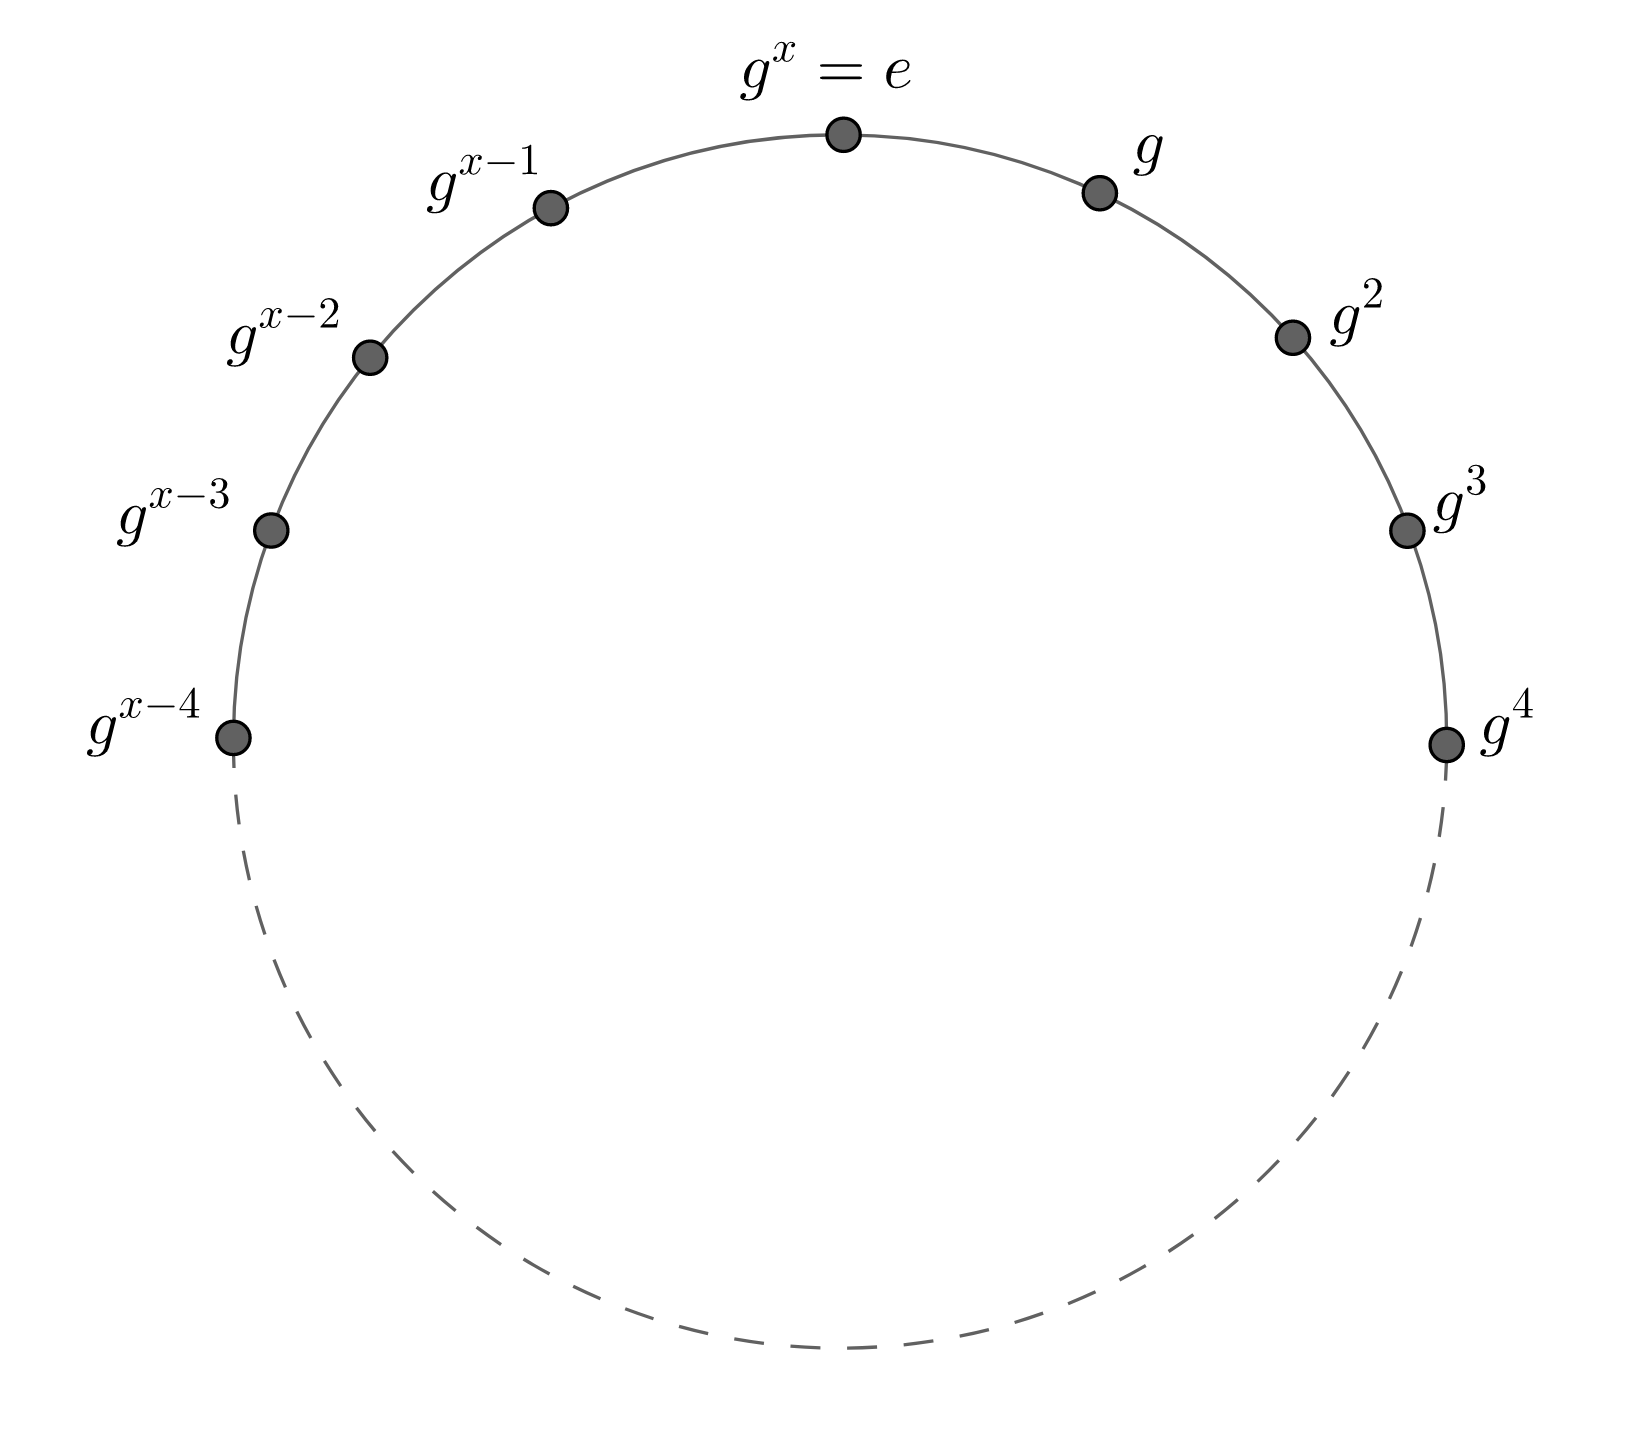
\includegraphics[width=.6\linewidth, height=.67\textheight, keepaspectratio]{Figures/cyclicgroup}
\caption{Cyclic group\index{cyclic group}\index{group}}
\label{Cyclic group}
\end{center}
\end{figure}

A a well known practice of presenting a finite group's\index{group} operation is {\em Cayley table\index{Cayley table}} as shown in example \ref{example_Cayleytable}.
Cayley table\index{Cayley table} shows all possible group operation that can be performed in a finite group.

\begin{example} \label{example_Cayleytable}
	The Cayley table\index{Cayley!Cayley table} for the group\index{group} $\mathbb{Z}_4$ is:
	\begin{center}
		\begin{tabular}{c|cccc}
			$\oplus_4$&\em 0&\em 1&\em 2&\em 3       \\
			\hline
			\em 0&\em 0&\em 1&\em 2&\em 3       \\
			\em 1&\em 1&\em 2&\em 3&\em 0       \\
			\em 2&\em 2&\em 3&\em 0&\em 1       \\
			\em 3&\em 3&\em 0&\em 1&\em 2       \\
		\end{tabular}
	\end{center}
\end{example}
In the above example of group $(\mathbb{Z}_4,+)$, there are $\phi(4)=2$ generators, $3$ and $1$.

\begin{definition}[Subgroup\index{subgroup}]
	Let $\mathbb{H}$ be  a non-empty subset  fo group $\mathbb{G}$, $\mathbb{H}$  will be called subgroup of $\mathbb{G}$ if  $\mathbb{H}$  itself follows group axioms and $\mathbb{H}$ has the same identity element of group $\mathbb{G}$. 
	\qed
\end{definition}

\begin{theorem}[Lagrange's Theorem:]
	Let $\mathbb{G}$ be a finite abelian group and $\mathbb{H}$ is a subgroup of $\mathbb{G}$.  The order of $\mathbb{G}$, $\#\mathbb{G}$ is divisible by the order of subgroup $\mathbb{H}$, $\#\mathbb{H}$ i.e.   $\#\mathbb{H} | \#\mathbb{G}$.
\qed
\end{theorem}

\begin{theorem}[Fermat’s Little Theorem:]
	Let $p$ is a prime and $a \in \mathbb{Z}$, then $$a^p = a ~(\bmod ~p)$$
	\qed
\end{theorem}
Fermat’s \textit{little theorem} is a special case of Lagrange’s theorem.


\subsection{Homomorphism in groups \index{homomorphism}}
Morphisms in groups is often used the research of cryptography and inseparable to for pairing-based cryptography research.
\begin{definition}[Homomorphism\index{rings}]
	Let $(\mathbb{G},\circ)$ and $(\mathbb{G}^{'},\star)$ be two groups with identity elements $e$ and $e'$ respectively.
	A homomorphism  is a map $f$ which preserves the group structure while the elements are mapped from $(\mathbb{G},\circ)$ to $(\mathbb{G}^{'},\star)$.
	\qed
\end{definition}
	A homomorphic map obeys the following conditions:
	\begin{itemize}
		\item $\forall a,b \in \mathbb{G}$, $f(a \circ b) = f(a) \star f(b)$.
		\item  For every $a \in \mathbb{G}$, the inverse map is $f(a^{-1}) = f(a)^{-1}$.
		\item  Identity element mapping also preserves the structure i.e. $f(e) =e'$.
	\end{itemize}

\subsubsection{Types of Homomorphism}
\begin{quote}
	\begin{description}
				\item[Isomorphism \index{Isomorphism}] If element from $\mathbb{G}$  and $\mathbb{G}^{'}$ have bijective relation then $\mathbb{G}$ and $\mathbb{G}^{'}$ are isomorphic to each other.
					
			\item[Endomorphism  \index{Endomorphism}]  If elements from group $(\mathbb{G},\circ)$ is mapped to itself then it is called endomorphism. 
			A frequently used endomorphism in cryptographic algorithms is Frobenius endomorphism. 
			
			\item[Authomorphism  \index{Authomorphism}] If element of a group has both endomorphism and isomorphism then it is called automorphism.
	\end{description}
\end{quote}

\begin{definition}[Kernel\index{kernel}]
	Let $(\mathbb{G},\circ)$ and $(\mathbb{G}^{'},\star)$ be two groups with identity elements $e$ and $e'$ respectively and $f$ is homomorphism from $(\mathbb{G},\circ)$ to $(\mathbb{G}^{'},\star)$.
	The kernel of $f$ is denoted as $\text{Ker}\{f\}$, defined by 
	$$\text{Ker}(f) = \{ a \in \mathbb{G}: f(a) = e'\}$$.
	\qed
\end{definition}

%--------------------------------------
%--------------------------------------
\subsection{Ring}
The concept of \textit{Ring} will not come as frequently as group and field in the subsequent chapters. 
However, it is relevant to define ring to understand the related concept.
\begin{definition}[Ring \index{ring}]
	A \textbf{ring} $\mathbb{R}$ is an algebraic structure with two operations, i.e. addition  $+$ and  multiplication $\cdot$  usually denote as $\mathbb{R},+,\cdot$.
	\begin{itemize}
		\item $\mathbb{R}$ is abelian group under addition operation.
		\item Under multiplication, $\mathbb{R}$ is closed and associative with identity element is $1$.
		\item  Multiplication is distributive over addition: $ \forall a, b, c \in \mathbb{R}: a\cdot (b+c) = a\cdot b + a\cdot c$.
	\end{itemize}
\qed
\end{definition}
If multiplication operation is commutative, $\mathbb{R}$  forms a commutative ring.
%\begin{example}
%	TODO
%\end{example}
\begin{definition}[Multiplicative Inverse Modulo $n$ \index{multiplicative inverse}]
	Let $\mathbb{Z}_n$ be a set under modulo $n$ and $a \in \mathbb{Z}_n$. 
	The multiplicative inverse modulo $n$ of $a$ can be written as  follows:
	$$a\cdot x \equiv  1 \bmod n.$$
The value $x$ is the multiplicative inverse modulo $n$ of $a$, often written as $a^{-1}$.
\qed
\end{definition}
Such value of $x$ only exists if $\text{gcd}(x,n)=1$.
If $n=p$ is a prime then every non-zero element in the set $\mathbb{Z}_p$ will have multiplicative inverse.
Such $(\mathbb{Z}_p,+,\cdot)$ will be a ring and having the above property it will form a field.

\subsection{Field}
\begin{definition}[Field]
	A field $(\f{},+,\cdot)$ is a set that obeys two binary operations denoted by $+$ and $\cdot$, such that:
	\begin{itemize}
%		\begin{itemize}
			\item $\f{}$ is a commutative group with respect to $+$ having identity element $0$.
			
			\item Let ${\f{\,}}^{\ast}\!\!$ is a subset of $\f{}$ having only not-zero element of $\f{}$ i.e. ${\f{}}^{\ast}  = {\f{} ~\backslash \{0\}}$. 
			Then ${\f{\,}}^{\ast}\!\!$ will be called a commutative group respect to multiplication$\cdot$  where every element should have multiplicative inverse in  ${\f{\,}}^{\ast}\!\!$.
			\item For all $a,b,c \in\f{}$  the distributive law will be followed, e.g. $a\cdot(b+c)=a\cdot b+a\cdot c$ and $(b+c)\cdot a=b\cdot a +c\cdot a$.
	\end{itemize}
%\end{itemize}
	\qed
\end{definition}
%In general, the elements $0$ and $1$ denote the unit elements regarding to addition $+$ and multiplication $\cdot$, respectively.
\begin{definition}[Subfield \index{subfield}]\hspace{0em} \label{definition_subfielf}
	Let $\f{1}$ is a subset of field $\f{}$. $\f{1}$ will be called a subfeld if $\f{1}$ itself obeys the laws of field with respect to the field operation inherited from  $\f{}$.
	\qed
\end{definition}
\begin{remark}
	 In Definition \ref{definition_subfielf}, $\f{}$ is called an {\em extension field} of $\f{1}$.
	  If $\f{1}\neq \f{}$, then $\f{1}$ is a {\em proper subfield} of $\f{}$.
 \end{remark}

\begin{definition}[Order of Finite Field \index{order of field}]\hspace{0em}
	The order is the number of elements in $\f{}$. If the order of $\f{}$ is finite, $\f{}$ is called finite field. 
	\qed
\end{definition}
\begin{definition}[Characteristic of Finite Field \index{field characteristics}]\hspace{0em}
	Let $\f{}$ be a field and smallest positive number $n$ such that $n \cdot a= 0$ for every $a\in \f{}$. Such $n$ is called characteristic. If there is no such $n$ in  $\f{}$ then $\f{}$ has characteristics $0$.
	\qed
\end{definition}

Most of the works presented in this dissertation deals with  finite fields only. 
A common property of finite fields often used in cryptographic is fllows:
\begin{theorem}\label{Cyclic Group in Finite Field}
	For every finite field $\f{}$, the multiplicative group $({\f{\,}}^{\ast}\!\!, \cdot)$ is cyclic. 
	\qed
\end{theorem}
%For example, ElGamal encryption \cite{C:ElGamal84} can be defined over multiplicative group of $\f{}$. Its security depends on the difficulty of a problem in $\f{}$ related to computing {\em discrete logarithms}.
%A subset $\mathbb K$ of a field $\f{}$ that is itself a field under the operations of $\f{}$ will be called a {\em subfield} of $\f{}$. In this case, $\f{}$ is called an {\em extension (field)} of $\mathbb K$. If $\mathbb K\neq \f{}$, we say that $\mathbb K$ is a {\em proper subfield} of $\f{}$. Then, {\em prime field} is defined as follows.
\begin{definition}[Prime Field \index{prime field}]
	Let $p$ be a prime. The ring of integers modulo $p$ is  a finite field of characteristics $p$ having field order $p$ denoted as $\f{p}$ is called a prime field.
	 \qed
\end{definition}
\begin{remark}
		A prime field contains no proper subfield.
\end{remark}

\begin{theorem}
	Every finite field has a prime field as a subfield. \qed
\end{theorem}

In this work we classified finite fields into two types, i.e.  prime field $\f{p}$ and its extension field. 
Defined \ref{sec:chap:fund:extenion_field} explains more of extension field.
The prime field $\Fp$ has  the order and characteristic as $p$.
Using the modular arithmetic in the same way as Definition \ref{sec:chap:fund:extenion_field}, we can define fundamental operations of prime field $\Fp=\{0,1,2\cdots,p-1\}$.
The Cayley table will de
\begin{example}The Cayley table for the two operations $+$ and $\cdot$ for elements in $\f{5}$ are as follows:
	\begin{center}
		\begin{tabular}{c|ccccc}
			$+$&\em 0&\em 1&\em 2&\em 3&\em 4       \\
			\hline
			\em 0&\em 0&\em 1&\em 2&\em 3&\em 4       \\
			\em 1&\em 1&\em 2&\em 3&\em 4&\em 0      \\
			\em 2&\em 2&\em 3&\em 4&\em 0&\em 1      \\
			\em 3&\em 3&\em 4&\em 0&\em 1&\em 2      \\
			\em 4&\em 4&\em 0&\em 1&\em 2&\em 3      \\
		\end{tabular}\ \ 
		\begin{tabular}{c|ccccc}
			$\cdot$&\em 0&\em 1&\em 2&\em 3&\em 4       \\
			\hline
			\em 0&\em 0&\em 0&\em 0&\em 0&\em 0       \\
			\em 1&\em 0&\em 1&\em 2&\em 3&\em 4      \\
			\em 2&\em 0&\em 2&\em 4&\em 1&\em 3      \\
			\em 3&\em 0&\em 3&\em 1&\em 4&\em 2      \\
			\em 4&\em 0&\em 4&\em 3&\em 2&\em 1      \\
		\end{tabular}
	\end{center}
\end{example}
As described above, we can define arithmetic operations in $\Fp$ by modular operations ($\bmod\ p$) for integers. However, it does not work in an extension field $\F{p}{m}$. In the next section, arithmetic operations in extension field $\F{p}{m}$ is described in detail.


\section{Extension Field} 
%\label{sec:chap:fund:extenion_field}
\label{sec:chap:fund:extenion_field}
%--------------------------------------
A subset $\F{0}{}$ of a field $\F{}{}$ that is itself a field under the operations of $\F{}{}$ will be called a {\it subfield} of $\F{}{}$.
In this case, $\F{}{}$ is called an {\it extension field} of $\F{0}{}$.
An extension field of a prime field $\F{p}{}$ can be represented as $m$-dimensional vector space that has $m$ elements in $\F{p}{}$.
Let the vector space be the $m$-th extension field, it is denoted by $\F{p}{m}$.
The order of extension fields $\F{p}{m}$ is given as $p^m$. 
In what follows, let $q$ be the power of $p$, the extension field of a prime field $\F{p}{}$ is denoted by $\F{q}{}$.



There are several methods to represent an element in extension fields, such as polynomial basis and normal basis.
In this thesis, we use normal basis.
Let $\omega$ be a root of $m$-th irreducible polynomial over $\F{q}{}$, we consider the following $m$ elements.

\begin{equation}
\omega,\;\omega^q,\;\omega^{q^2},\;\cdots,\;\omega^{q^{m-1}} \nonumber
\end{equation}
All elements in this set are conjugate to each other.
When the set of the conjugates become linearly independent, this is called {\it normal basis}.
Using normal basis, an element $\alpha \in \F{q}{}$ is expressed as a polynomial by  
\begin{equation}
\alpha = a_1 \omega + a_2 \omega^q + a_3 \omega^{q^2} + \cdots + a_m \omega^{q^{m-1}}, 
\end{equation}
where $a_1,\;a_2,\;a_3,\cdots,\;a_m \in \F{q}{}$.

Arithmetic operations in $\F{q}{m}$ are carried out with ordinary addition and multiplication for polynomial and modular reduction by irreducible polynomial.

\section{Frobenius Map}
\label{sec:chap:fund:frobeniusmap}
%--------------------------------------

For any element $\alpha \in \F{q}{m}$, let us consider the following map $\pi_q:\alpha \rightarrow \alpha^q$. 
%$\F{q}{m}$‚Ì”CˆÓ‚ÌŒ³$\alpha$‚ɑ΂µ‚Ä$\pi_q:\alpha \rightarrow \alpha^q$‚Æ‚¢‚¤ŽÊ‘œ‚ðl‚¦‚éD
\begin{eqnarray}
\pi_q(\alpha) &=& \left( a_1 \omega + a_2 \omega^q + a_3 \omega^{q^2} + \cdots + a_m \omega^{q^{m-1}} \right)^q \nonumber \\ 
&=& a_1 \omega^q + a_2 \omega^{q^2} + a_3 \omega^{q^3} + \cdots + a_m \omega^{q^m} \nonumber \\
&=& a_m \omega + a_1 \omega^q + a_2 \omega^{q^2} + \cdots + a_{m-1} \omega^{q^{m-1}}
\end{eqnarray}
Note that the order of $\F{q}{m}^*$ is given by $q^m - 1$, that is,  $\omega^{q^m} = \omega$ is satisfied.
Furthermore, $a^q$ is equal to $a$ for each coefficients $a$.

Therefore, the map $\pi_q(\alpha)$ is efficiently calculated by cyclic shift operations among its basis coefficients, 
which is free from arithmetic operations.
From the computational efficiency, the map $\pi_q$ is especially called Frobenius map.

In ElGamal Encryption, many exponentiations are executed in encryption and decryption processes.
When the exponent is equal to $p$, its calculation cost can be reduced by using Frobenius map.
Therefore, Frobenius map is widely used in the cryptographic application.     

\section{Quadratic Residue/Quadratic Non-residue, \\and Cubic Residue/Cubic Non-residue}
\label{sec:chap:fund:qrqnr}
%--------------------------------------

For any non-zero element $d\in\F{q}{}$, $d$ is called a Quadratic Residue (QR) when $x$ such that $x^2=d$ exists in $\F{q}{}$.
On the other hand, when such an $x$ does not exist in $\F{q}{}$, $d$ is called a Quadratic Non-Residue (QNR).
We can identify whether or not $d$ is a QR by following test.
%$\f{q}$‚Ì”CˆÓ‚Ì”ñ—댳$d$‚ɑ΂µC$x^2=d$‚Æ‚È‚é$x$‚ª$\f{q}$‚É‘¶Ý‚·‚é‚Æ‚«C$d$‚𕽕ûè—]iQuadratic Residue; QRj‚Æ‚¢‚¢C
%‘¶Ý‚µ‚È‚¢‚Æ‚«•½•û”ñè—]iQuadratic Non-Residue; QNRj‚Æ‚¢‚¤D‚»‚Ì”»•Ê‚ÍŽŸŽ®‚É‚æ‚ès‚¦‚éD
\begin{eqnarray}
d^{(q-1)/2} = \left\{
\begin{array}{ll}
1 & \mbox{: QR} \\
-1 & \mbox{: QNR} 
\end{array}
\right.
\end{eqnarray}

All elements in finite fields $\F{q}{}$ of odd characteristics become QR in extension fields $\F{q}{2j}$.
On the other hand, quadratic non-residues also become QNR in $\F{q}{i}$, where $i$ is not divisible by 2.

%%%%%%%%%%%%%%%%%%%%%%%%%%%%%%%%%%%%%%%
\section{Elliptic Curve}
\label{sec:chap:fund:ecc}
In this section, we review elliptic curves and pairings. 

%--------------------------------------
\subsection{Additive Group over Elliptic Curves}
%--------------------------------------

In general, let $p>3$, an elliptic curve $E/\F{p}{}$ over a finite field $\F{p}{}$ is defined as 

\begin{equation}
E/\F{p}{}: y^2=x^3+ax+b,\ 42a^3+27b^2 \neq 0,\ a,b\in \F{p}{}. \label{EC}
\end{equation}

The field that $x$ and $y$ belong to is called the definition field. 
The solutions $(x,y)$ of \eqref{EC} is called rational points.
$E(\F{q}{})$ that is the set of rational points on the curve, including the {\it point at infinity} $\mathcal{O}$, forms an additive abelian group. 
The {\it point at infinity} works as an unity element in $E(\F{q}{})$.
When the definition field is $\F{q}{m}$, we denote the additive group by $E(\F{q}{m})$.

For rational points $P_1(x_1,y_1)$, $P_2(x_2,y_2)$ $\in E(\F{q}{})$, the elliptic curve addition $P_3(x_3,y_3)=P_1+P_2$ is defined as follows.
\begin{eqnarray*}
	\lambda &=& \left\{ \begin{array}{ll}
		{\displaystyle \frac{y_2-y_1}{x_2-x_1}} & P_1\neq P_2,\ x_1\neq x_2 \\
		& \\
		{\displaystyle \frac{3x_1^2+a}{2y_1}} & P_1=P_2 \\
		
	\end{array} \right.\\
	x_3 &=& \lambda^3-x_1-x_2\\
	y_3 &=& (x_1-x_3)\lambda-y_1
\end{eqnarray*} 
%In the case of $P_1=P_2$, the addition is especially called elliptic curve doubling. 
$\lambda$ is the tangent at the point on the curve and $\cal O$ is the additive unity in $E(\f{p})$.
In what follows, If $P_1 \neq P_2$ then $P_1+P_2$ is called elliptic curve addition (ECA). 
If $P_1=P_2$ then $P_1+P_2=2P_1$, which is known as elliptic curve doubling (ECD). 
%Let $\#E(\F{p}{})$ be its order, consider a large prime $r$ that divides $\#E(\F{p}{})$. %The smallest positive integer $k$ such that $r$ divides $p^k-1$ is called {\it embedding degree}. One can consider pairings such as Tate and Ate pairings by using $E(\F{p}{k})$. 

Let a rational point $P(x,y)$, an inverse point $-P$ is given by $-P(x, -y)$. 
Elliptic curve cryptographies is constructed on elliptic curve groups $E(\F{q}{})$.



Let $\#E(\F{p}{})$ be the order of $E(\F{p}{})$, it is given as
\begin{equation}
\#E(\F{p}{})=p+1-t, %abel{order}
\end{equation}
where $t$ is the Frobenius trace of $E(\F{p}{})$. 

From Hasse's theorem, $t$ satisfies
\begin{equation}
|t| \leq 2\sqrt{p}.
\end{equation}

\subsection{Scalar Multiplication in Elliptic Curve}
\label{sec:chap:fund:scm}
Let $[s]P$ denote the $(s-1)$-times addition of a rational point $P$ as, 
\begin{equation}
[s]P = \sum_{i = 0}^{s-1}{P}.
\end{equation}
This operation is called a scalar multiplication.
As a general approach for accelerating a scalar multiplication, the binary method is the most widely used.

\paragraph{Binary method}
\label{sec:chap:fund:binscm}
The binary method is an extensively applied method for calculating the elliptic curve scalar multiplication. 
 The pseudo code of left-to-right binary scalar multiplication algorithm is shown in \algref{alg:binary_scm_chap_fundamental}. 
 This algorithm scans the bits of scalar $s$ from the  most significant bit to the least significant bit. When $s[i] = 1$, it  performs ECA and ECD otherwise only ECD is calculated. 
 The binary method iterates elliptic curve doublings and elliptic curve additions using binary representation of scalar.
 A scalar multiplication needs $\lfloor \log_2 s\rfloor$ elliptic curve doublings and $\lfloor \log_2 s\rfloor/2$ elliptic curve additions on average.
  This method is easy to implement but the important drawback of this method is not resistant to \textit{side channel attack} \cite{C:Kocher96}.  

\begin{algorithm}[ht]
	\caption{Left-to-right binary algorithm for elliptic curve scalar multiplication}
	\label{alg:binary_scm_chap_fundamental}
	\DontPrintSemicolon
%	\hspace{-3ex}
	\KwIn{ $P$, $s$}
%	\hspace{-3ex}
	\KwOut{$[s]P$} %output
	 $T$ $ \leftarrow$ $0$ \;
	 \For{$i = \lfloor \log_2 s \rfloor$ {\bf to} $0$} {\;
				$T \leftarrow T  + T$\;
		    \If{ $s[i] = 1$}{
			      $ T \leftarrow T + P$\;
	} }
	 \text{return} $T$\;
\end{algorithm}

\paragraph{Montgomery ladder method}
\label{sec:chap:fund:montscm}
Montgomery ladder algorithm is said to be resistant to \textit{side channel attack}. Such resistance comes by paying tolls as calculation overhead which slows down this method than binary method.  \algref{alg:mont_scm_chap_fundamental} shows the Montgomery ladder algorithm for scalar multiplication. Montgomery ladder has some similarity with binary method except in each iteration it performs ECA and ECD. 

\begin{algorithm}[ht]
	\caption{Montgomery ladder algorithm for elliptic curve scalar multiplication}
	\label{alg:mont_scm_chap_fundamental}
	\DontPrintSemicolon
%	\hspace{-3ex}
	\KwIn{ A point $P$,  an integer $s $}
%	\hspace{-3ex}
	\KwOut{$[s]P$} %output
	 $T_0$ $ \leftarrow$ $0$, $T_1$ $\leftarrow$ $P$ \;
	 \For{$i = \lfloor \log_2 s \rfloor$ {\bf to} $0$} {\;
		  \If{ $s[i] =1$}{
			         $ T_0 \leftarrow T_0 + T_1$\;
			     $T_1 \leftarrow T_1 + T_1$\;
		}
		        {\ElseIf{$s[i] = 0$}{ 
				      $T_1 \leftarrow T_0 + T_1$\;
				  		 $T_0 \leftarrow T_0 + T_0$\;}
		}
	}
	 \text{return} $T_0$\;
\end{algorithm}

\paragraph{Sliding-window Method}
\label{sec:chap:fund:swscm}
Sliding-window \cite{DBLP:reference/crc/2005ehcc} algorithm is also resistant to \textit{side channel attack} and at the same  time it is faster than Montgomery ladder. In this method the scalar $s$ is processed in blocks of length $w$, known as window size. \algref{alg:sw_scm_chap_fundamental} shows the sliding-window algorithm for scalar multiplication.

\begin{algorithm}[ht]
	\caption{Sliding window algorithm for elliptic curve scalar multiplication}
	\label{alg:sw_scm_chap_fundamental}
	\DontPrintSemicolon
%	\hspace{-3ex}
	\KwIn{ A point $P$,  an integer $s = \sum_{j=0}^{l-1} s_j2^{j} $, $s_j \in \left\lbrace 0,1 \right\rbrace$, window size $w \geq 1$} 
%	\hspace{-3ex}
	\KwOut{Q = $[s]P$} 
	\textit{Pre-computation.} \; 
	 $P_1\leftarrow P$, $P_2 \leftarrow [2]P$ \;
	 \For{$i = 1$ {\bf to} $2^{w-1}-1$} { $P_{2i+1} \leftarrow P_{2i-1} + P_2$}\;
	 $j \leftarrow l-1$, $Q \leftarrow \cal{O}.$\;
	\textit{Main loop.}\;
	 \While{$j \geq 0$} {\;
		 \If{ $s_j =0$}{
			$Q \leftarrow [2]Q$, $j \leftarrow j-1$\;
		}
		            \Else{\;
			 Let $t$ be the least ineger such that \;
			$j - t+1 \leq w$ and $s_t =1$\;
			 $h_j \leftarrow (s_js_{j-1} \cdots s_t)_2$\;
			 $Q \leftarrow [2^{j-t+1}]Q +P_{h_j}$      \;      
			 $j \leftarrow t-1$ \;
		}
	}
	 return $Q$
\end{algorithm}



%In this paper, the set of rational points $P\in E(\F{q}{})$ satisfying $[r]P=\mathcal{O}$ is denoted by $E(\F{q}{})[r]$.
%For two points $P$ and $R$ such that $[s]P=R$, the problem of solving $s$ is called elliptic curve discrete logarithm problem (ECDLP) and the security of ECC relies on the difficulty of ECDLP.

%\begin{figure}[ht]
%	\begin{center}
%		\special{pn 10}%
%		\special{ar 3150 950 700 700 0.1200000 0.14959965}
%		\special{ar 3150 950 700 700 0.2991993 0.44879895}
%		\special{ar 3150 950 700 700 0.5983986 0.74799825}
%		\special{ar 3150 950 700 700 0.8975979 1.04719755}
%		\special{ar 3150 950 700 700 1.1967972 1.34639685}
%		\special{ar 3150 950 700 700 1.4959965 1.64559615}
%		\special{ar 3150 950 700 700 1.7951958 1.94479545}
%		\special{ar 3150 950 700 700 2.0943951 2.24399475}
%		\special{ar 3150 950 700 700 2.3935944 2.54319405}
%		\special{ar 3150 950 700 700 2.6927937 2.84239335}
%		\special{ar 3150 950 700 700 2.9919930 3.02159265}
%		\special{ar 3850 950 80 80 0.000000000 6.283185304}
%		\special{ar 2450 950 80 80 0.000000000 6.283185304}
%		\special{ar 3150 250 80 80 0.000000000 6.283185304}
%		\special{ar 3500 355 80 80 0.000000000 6.283185304}
%		\special{ar 3745 600 80 80 0.000000000 6.283185304}
%		\special{ar 2555 600 80 80 0.000000000 6.283185304}
%		\special{ar 2800 355 80 80 0.000000000 6.283185304}
%		\special{ar 3150 950 700 700 3.261 3.555}
%		\special{ar 3150 950 700 700 3.79 4.065}
%		\special{ar 3150 950 700 700 4.3 4.591}
%		\special{ar 3150 950 700 700 4.83 5.122}
%		\special{ar 3150 950 700 700 5.365 5.63}
%		\special{ar 3150 950 700 700 5.87 6.165}
%		\begin{picture}(150,120)%
%		\put(50,115){$[\#E]P=\Inf$}
%		\put(110,100){$P$}
%		\put(128,80){$[2]P$}
%		\put(136,54){$[3]P$}
%		\put(-40,54){$[\#E-3]P$}
%		\put(-30,80){$[\#E-2]P$}
%		\put(-10,98){$[\#E-1]P$}
%		\end{picture}%
%	\end{center}
%	\caption{An image of elliptic curve group\index{cyclic group}\index{group}}
%	\label{fig:ECG}
%\end{figure}

%--------------------------------------
\subsection{Frobenius Map on Elliptic Curve Groups}
%--------------------------------------
In this section, we introduce Frobenius map for a rational point in $E(\F{q}{})$.
For any rational point $P=(x, y)$, Frobenius map $\phi$ is given by $\phi:P(x, y) \rightarrow ({x}^q, {y}^q)$.
Then, the following relation holds for any rational points in $E(\F{q}{})$ with regard to Frobenius map.
\begin{equation*}
\left(\phi^{2}-[t]\phi+[q]\right)P=\mathcal{O}.
\end{equation*}
Thus, we have
\begin{equation}
[q]P=\left([t]\phi-\phi^2\right)P. \label{frobscm}
\end{equation}
From Hasse's theorem, note the bit-size of Frobenius trace $t$ is about a half of the characteristic $p$. 
Using \eqref{frobscm}, we can efficiently calculate scalar multiplication \cite{C:Koblitz91}.
 
%\include{Chapters/Chapter3}
%\include{Chapters/Chapter4} 
%\include{Chapters/Chapter5} 

%----------------------------------------------------------------------------------------
%	THESIS CONTENT - APPENDICES
%----------------------------------------------------------------------------------------

\appendix % Cue to tell LaTeX that the following "chapters" are Appendices

% Include the appendices of the thesis as separate files from the Appendices folder
% Uncomment the lines as you write the Appendices

% Appendix A

\chapter{Frequently Asked Questions} % Main appendix title

\label{AppendixA} % For referencing this appendix elsewhere, use \ref{AppendixA}

\section{How do I change the colors of links?}

The color of links can be changed to your liking using:

{\small\verb!\hypersetup{urlcolor=red}!}, or

{\small\verb!\hypersetup{citecolor=green}!}, or

{\small\verb!\hypersetup{allcolor=blue}!}.

\noindent If you want to completely hide the links, you can use:

{\small\verb!\hypersetup{allcolors=.}!}, or even better: 

{\small\verb!\hypersetup{hidelinks}!}.

\noindent If you want to have obvious links in the PDF but not the printed text, use:

{\small\verb!\hypersetup{colorlinks=false}!}.

%\include{Appendices/AppendixB}
%\include{Appendices/AppendixC}

%----------------------------------------------------------------------------------------
%	BIBLIOGRAPHY
%----------------------------------------------------------------------------------------

\printbibliography[heading=bibintoc]

%----------------------------------------------------------------------------------------

\end{document}  
